% \part{Template}\label{part:appendices}
\chapter{Collective radiance in atomic arrays and volumes}\label{ch:collectiveradiance}

As originally explored by Dicke, two or more spins in proximity to each other will have their spontaneous emission rate modified due to interference\cite{Dicke1954}. His original thought experiment is presented in Fig. (\ref{fig:DickeNeutronDecay}) Such collective interactions can either enhance or suppress the spontaneous decay rate of many quantum emitters, compared to any individual emitter in isolation, depending on the spacing between the emitters as a fraction of the emission wavelength. In addtion to modified decay rates (or equivalently, excited state lifetimes), the emission pattern may be highly directional\cite{ballantine2020subradiance}, and the light even from a disordered ensemble of atoms may be exhibit spatial coherence \cite{gold2022spatial}. These emergent phenomena are of interest for many-body physics studies as well as potential applications in quantum technologies, such as for creating an "atomic antenna", efficiently mapping light into an optical fiber e.g. for quantum communication \cite{grankin2018free, jones2020collectively}.

\begin{figure}[!ht]
    \centering
    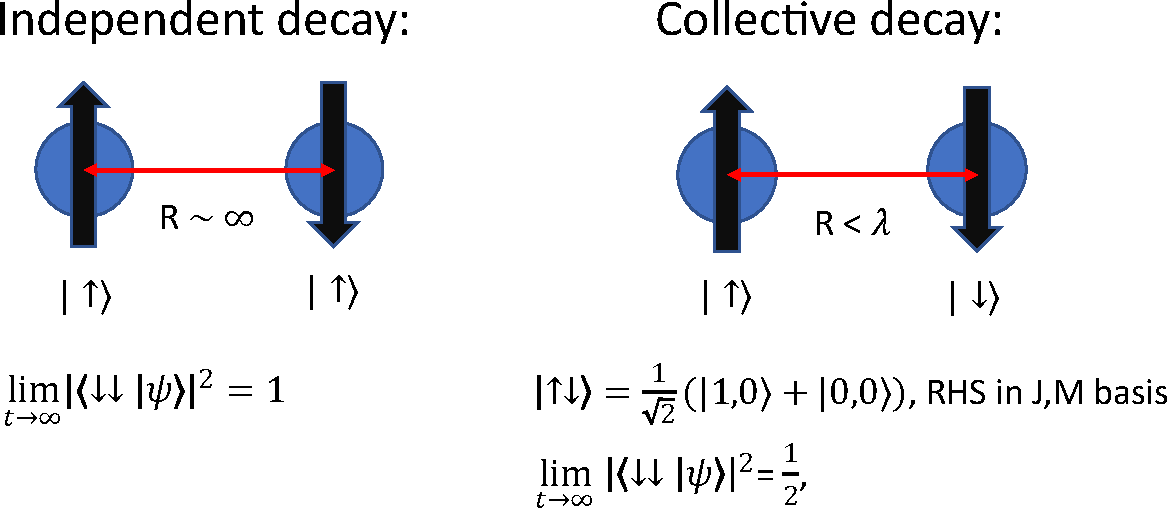
\includegraphics[width=0.9\textwidth]{Images/Dicke_neutron_decay.pdf}
    \caption{A pictorial representation of Dicke's simple explanation for the existence modified spontaneous decay rates using neutrons. In the case where two neutrons are far apart, their decay rates are unchanged and the probability to observe emission if one neutron is excited is unity if we wait long enough. For the case where the neutrons are sufficiently clsoe together, the state is now a superposition of a singlet and triplet state, and the emission probability is $1/2$.}
    \label{fig:DickeNeutronDecay}
\end{figure}

In what follows, we will give an overview of the physics of collective radiance effects in ordered arrays through a numerical study of the conditions in which they arise. We will also explore to what extent the interesting emergent features are sensitive to various imperfections in the atomic arrays. Numerous studies have been done to calculate various features of interest for different geometries \cite{moreno2019subradiance, ballantine2020subradiance, bettles2016enhanced} which may provide more detailed analysis than what is outlined here.

\section{Hamiltonian for the single-excitation subspace}

For two level atoms arranged in a 2D grid (Fig. (\ref{fig:2datomgrid})) interacting with an incident oscillating electric field near the tranisiton resonance, it is straightforward to write down the semi-classical system Hamiltonian. We will limit this analysis to the single-excitation subspace, meaning that the Hilbert space is truncated so there is at most one excitation $\hbar \omega_0$ in the array, where $\omega_0$ is the atomic transition angular frequency. 

\begin{figure}[!ht]
    \centering
    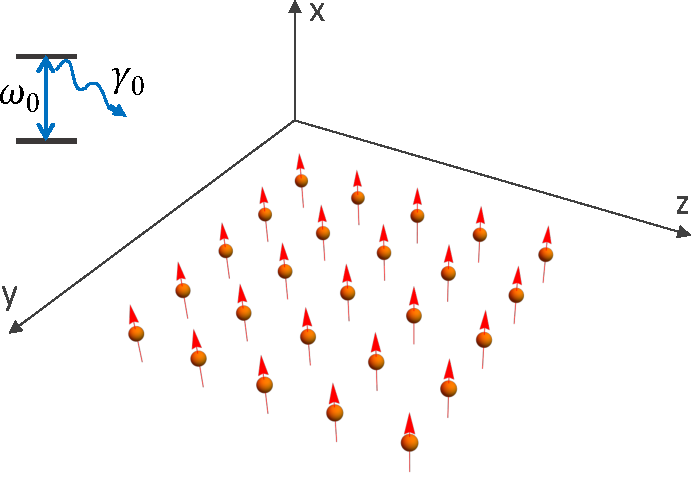
\includegraphics[width=0.45\textwidth]{Images/atomgrid.pdf}
    \caption{A 2D grid of two-level atoms, or equivalently, classical electric dipoles.}
    \label{fig:2datomgrid}
\end{figure}

The matrix elements of the effective dissipative Hamiltonian are given by
\begin{equation}\label{eq:greenham}
    \bra{1_i} H \ket{1_j} = H_{ij} = \Omega_{ij}(1 - \delta_{ij}) + i\gamma_{ij}\delta_{ij}
\end{equation}
where $\Omega_{ij}$ and $\gamma_{ij}$ are related to the Green's tensor and the states $\ket{1_i}$ are a shorthand for the state with only atom $i$ excited: 
\begin{equation}
    \ket{1_i} = \ket{0_0} \otimes \ket{0_1} \otimes ... \ket{1_i} ... \ket{0_{N-1}} \otimes \ket{0_N}
\end{equation}

The effective coupling and decay terms are given by the dipole-dipole interaction between radiating dipoles with orientations $e_{\mu}$ and $e_{\mu}$ for dipoles (atoms) at positions $r_i$ and $r_j$: 
\begin{equation}
    \Omega_{ij} + i \gamma_{ij} = \frac{6\pi \gamma}{k^3}\hat{e_{\mu}}\cdot G(\mathbf{r}_i - \mathbf{r}_j) \cdot \hat{e_{\nu}}
\end{equation}
where $G$ is the Green's tensor, giving
\begin{equation}
    \begin{aligned}
        G\left(\mathbf{r}\right) \cdot \hat{e}_{\nu}= & \frac{e^{i k r}}{4 \pi r}\left[(\hat{\mathbf{r}} \times \hat{e}_{\nu}) \times \hat{\mathbf{r}} \right. \\
        & \left.+\left(\frac{1}{k^2 r^2}-\frac{i}{k r}\right)\left(3 \hat{\mathbf{r}}(\hat{\mathbf{r}} \cdot \hat{e}_{\nu})-\hat{e}_{\nu}\right)\right]
    \end{aligned}
\end{equation}
where $k$ is the wavenumber. We can now investigate dynamics of such a system by numerically, including finding the eigenmodes by diagonalizing the Hamiltonian for various system geometries, as well as solving for temporal dynamics given an initial excitation in the array.

\section{Eigenmodes, decay, and emission patterns of 2D arrays}
For a square grid of atoms we can numerically diagonalize Eq. (\ref{eq:greenham}) to find the eigenvalues $\lambda_n$ where the collective Lamb shift $\delta_n$ and decay rate (linewidth) $\nu_n$ of the mode are given by the real and imaginary parts, respectively, of $\lambda_n$. For the dipole orientations we will restrict the system to a few different cases, all of which have $|e_{\mu}| = |e_{\nu}|$ and polarization aligned either perpendicular to or parallel with the plane in which the atoms live. For the perpendicular case, we will label the case of all dipole moments aligned as "symmetric", and "anti-symmetric" for the case where each dipole is $\pi$ out of phase with its neighbor (Fig. (\ref{fig:symm_antisymm_modes}))

\begin{figure}[!ht]
    \centering
    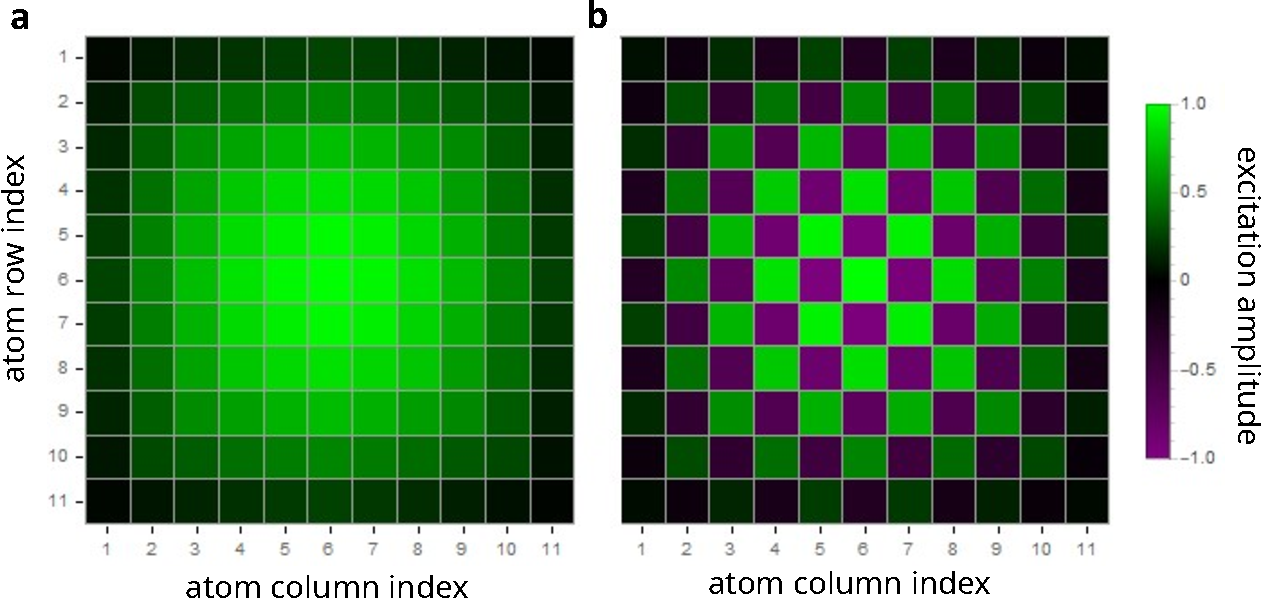
\includegraphics[width=0.9\textwidth]{Images/symm_anti_symm_modes.pdf}
    \caption{Symmetric (a) and anti-symmetric (b) modes of an 11x11 square grid of atoms with out-of-plane polarization, found by sorting the eigenmodes by maximum overlap with the state of interest.}
    \label{fig:symm_antisymm_modes}
\end{figure}

The linewidths for the symmetric states vary as a function of array spacing, where the suppression and enhancement compared to the natural linewidth can be thought of as a sort of two-dimensional cavity, where modulating the length in each direction brings the system into and out of resonance. Indeed, placing a single atom in a 1D cavity is directly analagous to placing it in a periodic array of atoms, where loosely speaking, a higher finesse cavity would correspond to an array with more atoms. The linewidths versus array spacing for different polarization orientations is shown in Fig. (\ref{fig:collective_linewidths_2d}), where the red circle emphasizes that four orders of magnitude linewidth suppression can be acheived with just 25 atoms. It is clear that for in-plane polarization the linewidth is close to or enhanced compared to natural linewidth, whereas there can be significant supression for polarization perpendicular to the plane. An intuitive explanation of this is arrived at by considering that the emission of linearly polarized radiation will propagate perpendicularly to the orientation of the dipole. Thus, for polarization perpendicular (parallel) to the atomic array, the radiation will propagate mostly in the (perpendicular to) plane of the array.

\begin{figure}[!ht]
    \centering
    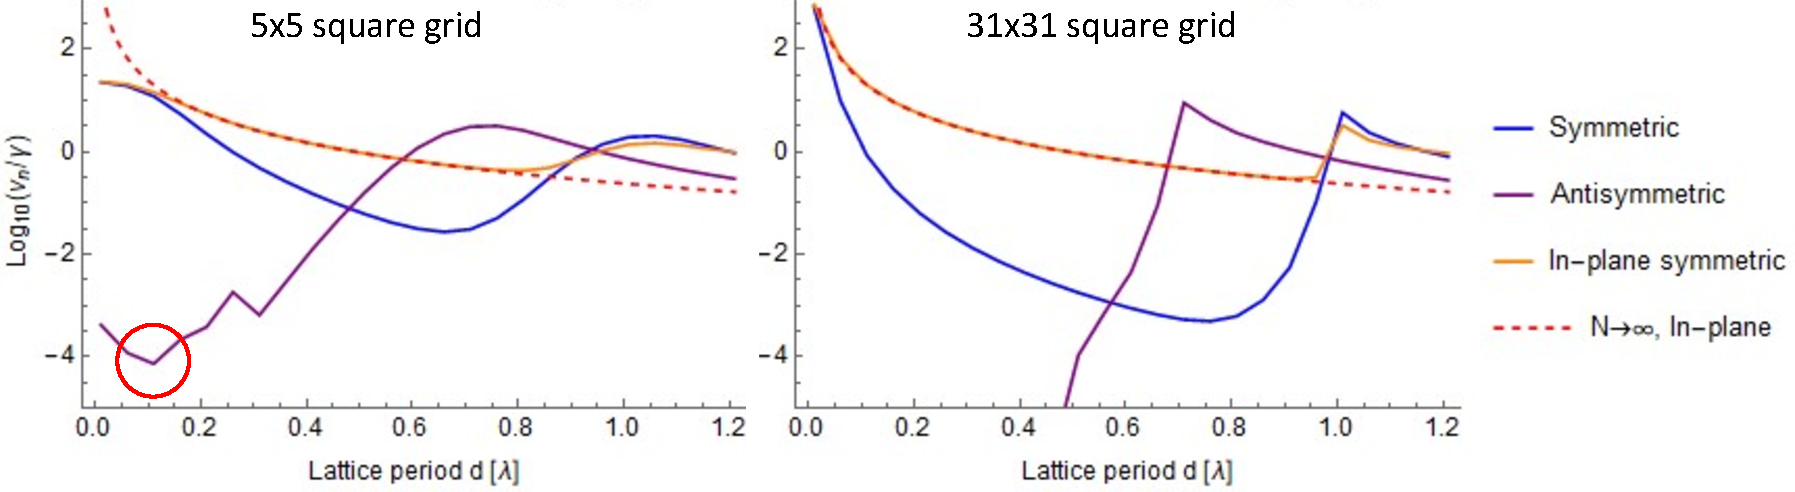
\includegraphics[width=0.9\textwidth]{Images/collective_linewidths_2d.pdf}
    \caption{Linewidths for various polarization orientations of atom arrays of two sizes. For the 31x31 array, the author has reproduced with his own code the results from Fig. (2) of \cite{ballantine2020subradiance} as a sanity check, and the obvious mimicry of plot styling is intentional for ease of comparison.}
    \label{fig:collective_linewidths_2d}
\end{figure}

In practice, creating a single excitation in an array to target a particular mode may be challening. As a case study, we consider a simple situation in which a 5-by-5 atom array is excited such with only the central 9 atoms targeted, each sharing the same share of the excitation (i.e., the amplitudes $|c_i|=1/3$).

We can compare symmetric and anti-symmetric excitation and analyze the mode overlap in time, as shown in Fig. (\ref{fig:collective_mode_decay_2d}), where the array period has been chosen to acheive subradiance in each case. The initial excitation does not perfectly overlap the desired eigenmode in either case, and it is clear that the superradiant components of the state decay quickly, until the remaining population is in the target state, which decays much more slowly than the natural decay rate.
\begin{figure}[!ht]
    \centering
    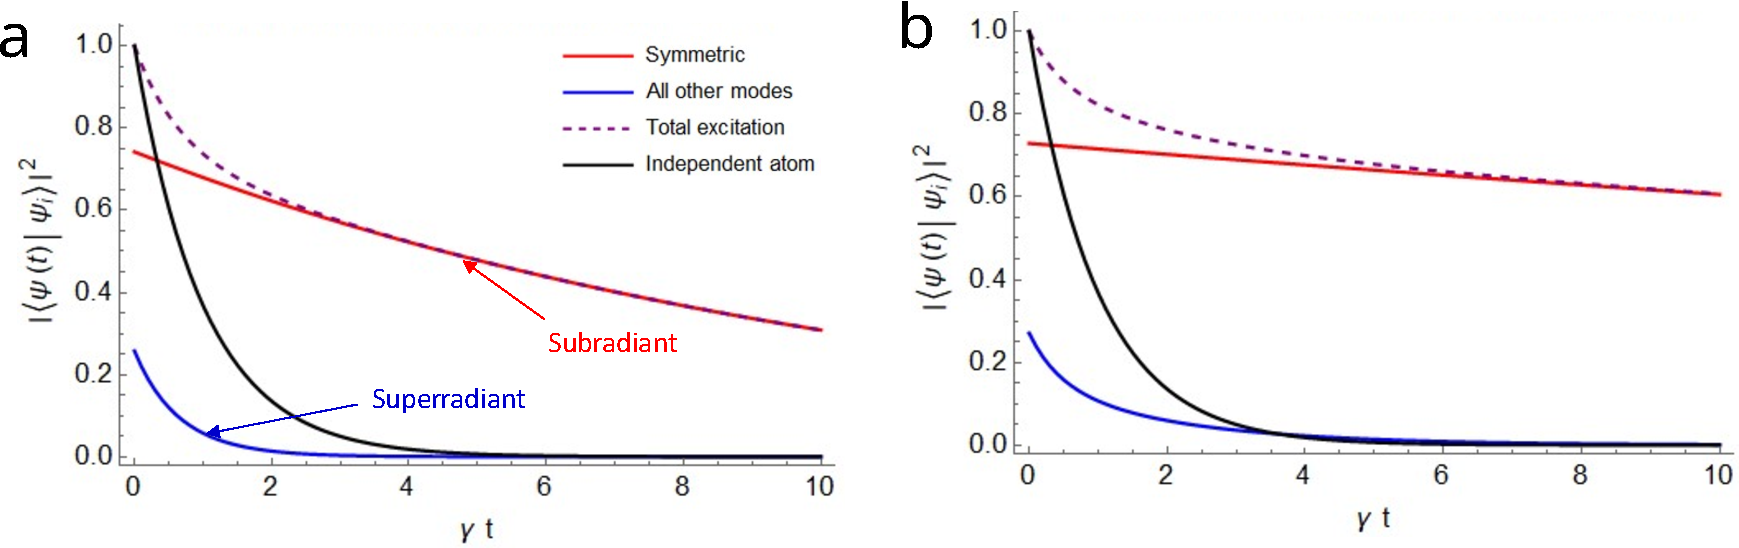
\includegraphics[width=0.9\textwidth]{Images/collective_decay_composition.pdf}
    \caption{Eigenmode composition of the excitation in the array versus time for an initial symmetric (a) and anti-symmetric excitation (b) of the 9 central atoms.}
    \label{fig:collective_mode_decay_2d}
\end{figure}

Intuition about the decay process can also be gained by analyzing snapshots of the emission pattern at different times for different excitation and polarization patterns. As shown in Fig. \ref{fig:collective_emission_patterns}, excitation with in-plane polarization decays quickly relative to the cases with polarization perpendicular to the plane. 
\begin{figure}[!ht]
    \centering
    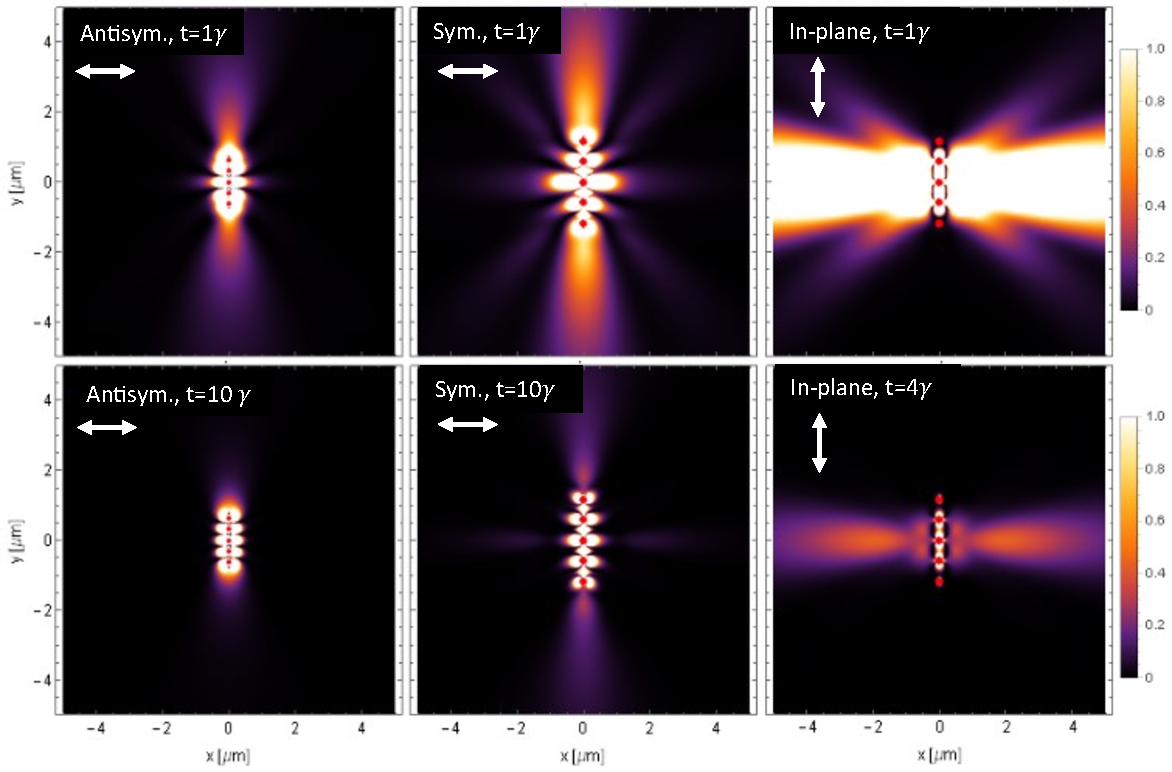
\includegraphics[width=0.9\textwidth]{Images/collective_emission_patterns.pdf}
    \caption{Emission intensity patterns at different times for different polarization arrangements, where the central nine atoms share a single excitation at $t=0$, i.e., $|c_i(t=0)|=1/3$ in all cases. The inset double arrow denotes the polarization direction.}
    \label{fig:collective_emission_patterns}
\end{figure}
The intuiton for this comes from considering the interference of emission directed along neighboring atoms, where, of course, there are only neighbors in-plane for a 2D grid. Remarkably, with only 25 atoms in a square monolayer we can already see highly directional emission for the case of in-plane polarization.

\section{Sensitivity to imperfections}

The modeling shown thus far assumed zero-temperature atoms frozen perfectly in place on a regular grid. In reality, finite temperature will lead to a spread in positions of the atoms giving a slight disordering of the array. For the case of polarization perpendicular to the atom plane, we are primarily concerned with in-plane positional spread and thus will neglect out-of-plane spread. The effect of in-positional deviation on decay suppression is shown for an 11-by-11 array in Fig. (\ref{fig:superradiance_vs_atomspread}), where the result from a Monte-Carlo simulation with 20 averages in which the atom's in-plane positions are pulled from Gaussian distributions of standard deviation $\sigma$.
\begin{figure}[!ht]
    \centering
    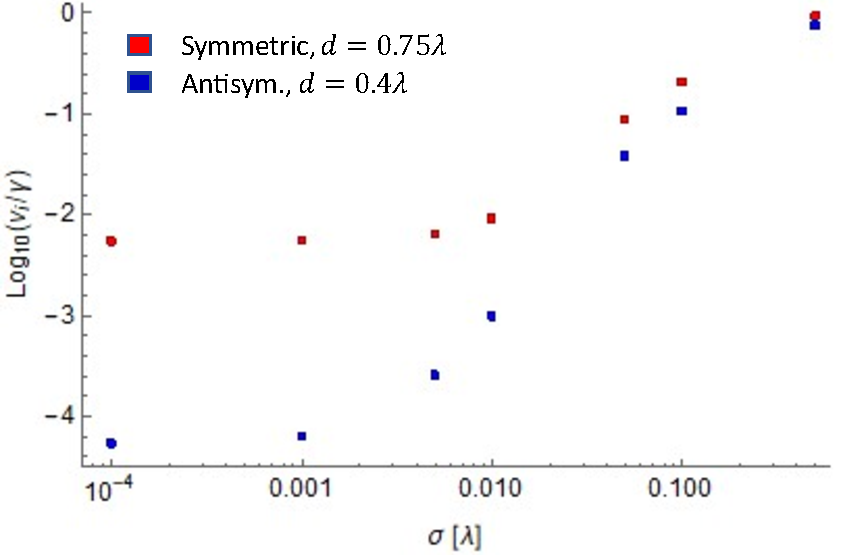
\includegraphics[width=0.45\textwidth]{Images/superradiance_vs_atom_spread.pdf}
    \caption{The collective decay rate for an 11-by-11 array versus the standard deviation of an atom's position in the plane of array, given by a Monte Carlo simulation.}
    \label{fig:superradiance_vs_atomspread}
\end{figure}
To give a practical foothold, an atom in an optical tweezer of waist and wavelength $w=\lambda=1~\mu$m, with temperature $1/5$ (e.g. 20 $\mu$K and 1 mK, respectively.)that of the trap, the transverse positional spread $\sigma_{\rho}$ is 0.1, from $\sigma_{\rho} = \sqrt{T_{\textrm{atom}}/(2T_{\textrm{FORT}})}$.
 
Another effect which will degrade the collective behavior is imperfect array filling, though creation of defect-free arrays can be accomplished through standard atom rearrangement techniques \cite{Ebadi2021}. The effect of defects is shown in Fig. (\ref{fig:superradiance_vs_eff}), again for an 11-by-11 array, with a Monte-Carlo simulation averaging over randomized defect placements for given array filling fractions.
\begin{figure}[!ht]
    \centering
    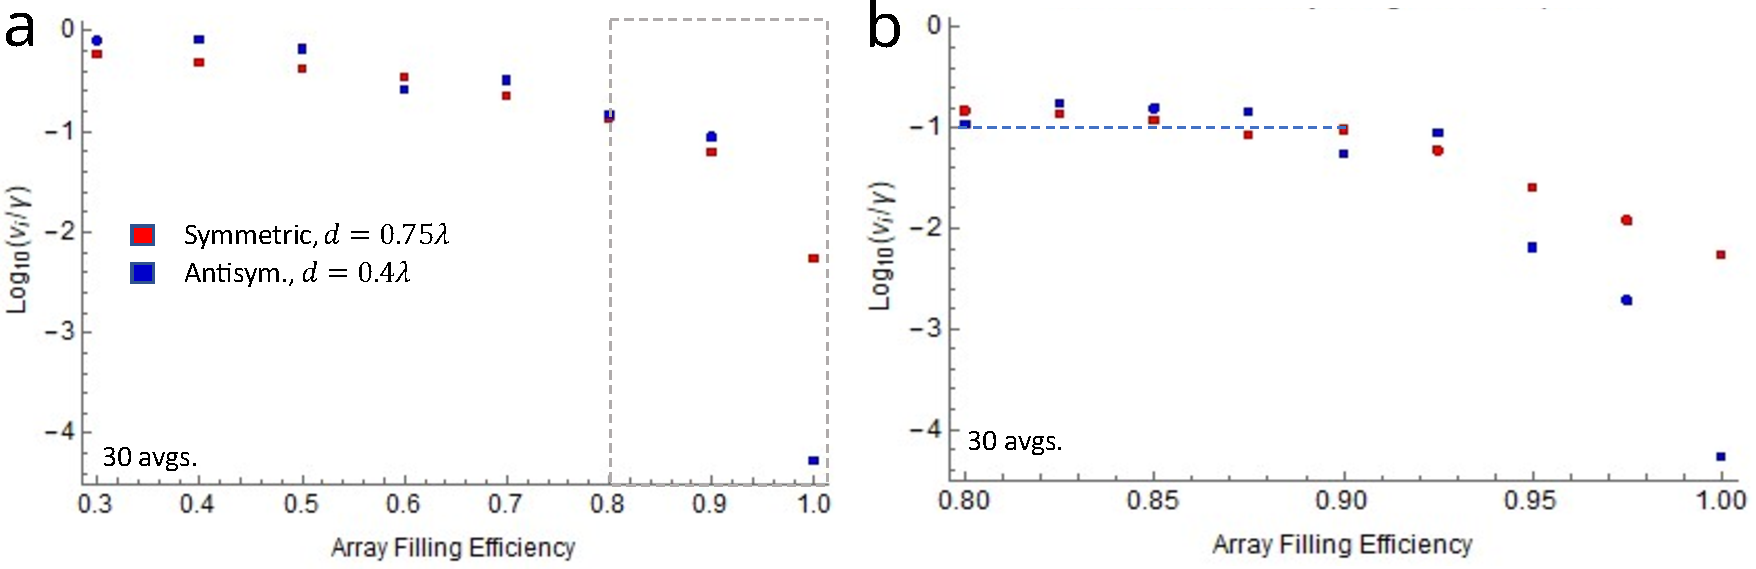
\includegraphics[width=0.9\textwidth]{Images/superradiance_vs_array_efficiency.pdf}
    \caption{The collective decay rate for an 11-by-11 array vs array filling fraction, given by a Monte Carlo simulation. (b) shows simulation results zoomed for more values of filling fraction over the range demarcated by the dashed box in (a). The dashed horizontal line in (b) is simply a guide to the eye.}
    \label{fig:superradiance_vs_eff}
\end{figure}

\section{Eigenmodes of 3D arrays}
The emergence of super- and subradiant states in planar arrays can be extended to a volume of atoms. This can enhance the effects discussed above and lead to new behaviors such as unidirectional or "chiral" emission\cite{grankin2018free}. Unsurprisingly, the addition of multiple atomic layers, where the array period is same in $x$, $y$, and $z$, can augment the supression or enhancement of the collective emission rate beyond what is observed for a single atomic layer as discussed in the previous section. This is shown for the symmetric singly-excited state in Fig. (\ref{fig:superradiance_volumetric}).
\begin{figure}[!ht]
    \centering
    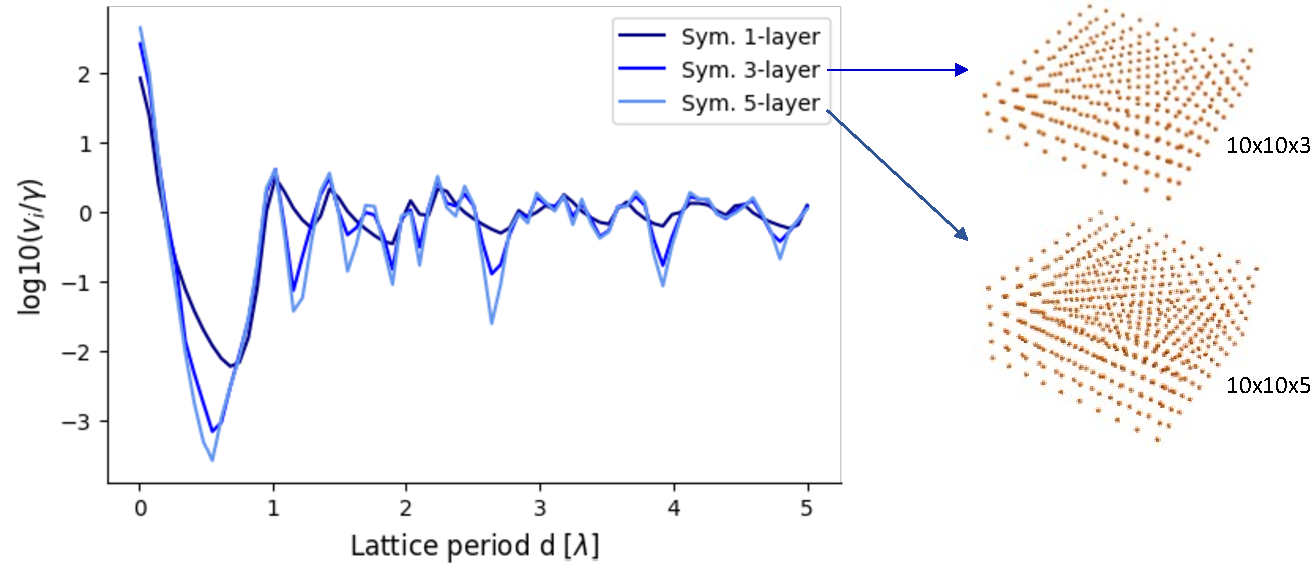
\includegraphics[width=0.9\textwidth]{Images/collective_radiance_in_volumetric_arrays.pdf}
    \caption{The collective decay rate of the symmetric state for a 1-, 3- and 5-layer atomic volume with 10
    $\times$10 atoms in the layers.}
    \label{fig:superradiance_volumetric}
\end{figure}
Typically, the discussion of collective radiance is limited to the so-called Dicke regime, where the characteristic spacing between emitters is less than the wavelength of the emitted radiation. However, we can see that for a volume of emitters, there is pronounced subradiance even for array periods larger than $\lambda$, and that this effect strengthens with additional atomic layers. 





